\documentclass{standalone}

\usepackage[euler-digits]{eulervm}

\usepackage{tikz}
\tikzset{every node/.style={draw=none,minimum size=6mm,inner sep=0pt}}

\begin{document}
    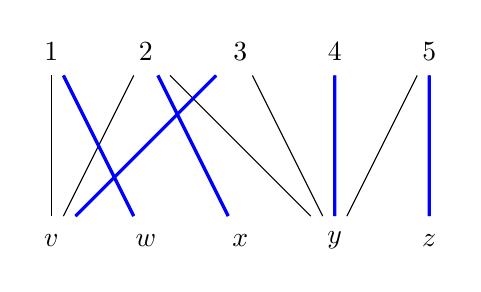
\begin{tikzpicture}[scale=1.2]
      \node (1) at (0,1) {$1$};
      \node (2) at (1,1) {$2$};
      \node (3) at (2,1) {$3$};
      \node (4) at (3,1) {$4$};
      \node (5) at (4,1) {$5$};
      \node (v) at (0,-1) {$v$};
      \node (w) at (1,-1) {$w$};
      \node (x) at (2,-1) {$x$};
      \node (y) at (3,-1) {$y$};
      \node (z) at (4,-1) {$z$};

\foreach \a/\b in {1/v,1/w,2/v,2/x,2/y,3/v,3/y,4/y,5/y,5/z}
  \draw (\a) -- (\b);
\foreach \a/\b in {1/w,2/x,3/v,4/y,5/z}
  \draw[blue,very thick] (\a) -- (\b);
    \end{tikzpicture}
\end{document}
